%path = ../Ex2/Informe/

\chapter{Celda Rauch (Deliyannis-Friend modificada}


Se buscó implementar un filtro pasa banda que cumpla con los parámetros indicados en el Cuadro \ref{tab:e2spec}.

\begin{table}[ht]
\begin{center}
\begin{tabular}{||c|c||}
\hline
Pendiente Pasabajos normalizado	&	$-40 \si{\deci\bel}/dec$ \\
\hline
$f_p$ & $56 \si{\kilo\hertz}$\\
\hline
$B$ & $1/10$\\
\hline
$A_p$ & $3\si{\deci\bel}$\\
\hline
$Z_{in}(f)$ & $\geq 50 \si{\kilo\ohm}$\\
\hline
\end{tabular}
\caption{Filtro Chebycheff}
\label{tab:e2spec}
\end{center}
\end{table}

\section{Transferencia Numérica}

A partir del dato de la pendiente del pasabajos normalizado, se determina que utilizando la aproximación de Chebycheff el orden del filtro será $n=2$. Aunque la amplitud máxima del filtro en banda pasante es $A_p = 3 \si{\deci\bel}$ se utilizó para el cálculo de la transferencia $A_p = 1$ ya que se previó que por las tolerancias de los componentes la curva de la transferencia se desplazará.

Usando la aproximación de Chebycheff para el filtro pasabajos normalizado y desnormalizándolo a un filtro pasabajos (véase Anexo), se obtuvo la expresión \eqref{eq:e2BP} de orden $n=4$.

\begin{equation}
H_{BP}(s)=\frac{1.2380\cdot10^9s^2}{s^4+3.8625\cdot10^4 s^3+2.4897\cdot10^{11}s^2+4.7819\cdot10^{15}+1.5328\cdot10^{22}}
\label{eq:e2BP}
\end{equation}

La plantilla resultante para este filtro se puede observar en la Figura \ref{fig:e2template}.

\begin{figure}[ht]
\begin{center}
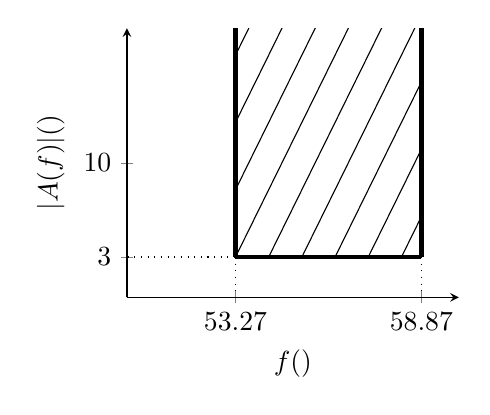
\begin{tikzpicture}
\begin{axis}[
    axis lines = left,
    xlabel = $f(\si{\kilo\hertz})$,
    ylabel = $|A(f)|(\si{\deci\bel})$,
    xmin = 50,
    xmax = 60,
    ymin = 0,
    ymax = 20,
    xtick = {0, 53.27, 58.87 },
    ytick = {3, 10 },
    height= 5cm
]
\addplot[
	domain=53.27:58.87,
	samples=10,
	color = black,
	ultra thick
] {3};
\addplot[domain=54.27:58.87,samples=10,color = black] {3+(x-54.27)*5};
\addplot[domain=55.27:58.87,samples=10,color = black] {3+(x-55.27)*5};
\addplot[domain=56.27:58.87,samples=10,color = black] {3+(x-56.27)*5};
\addplot[domain=57.27:58.87,samples=10,color = black] {3+(x-57.27)*5};
\addplot[domain=58.27:58.87,samples=10,color = black] {3+(x-58.27)*5};
\addplot[domain=53.27:58.87,samples=10,color = black] {3+(x-53.27)*5};
\addplot[domain=53.27:58.87,samples=10,color = black] {8+(x-53.27)*5};
\addplot[domain=53.27:58.87,samples=10,color = black] {13+(x-53.27)*5};
\addplot[domain=53.27:58.87,samples=10,color = black] {18+(x-53.27)*5};
\addplot[domain=53.27:58.87,samples=10,color = black] {23+(x-53.27)*5};
\addplot[domain=53.27:58.87,samples=10,color = black] {28+(x-53.27)*5};
\addplot[domain=53.27:58.87,samples=10,color = black] {33+(x-53.27)*5};
\addplot[domain=53.27:58.87,samples=10,color = black] {38+(x-53.27)*5};
\addplot[
	color=black,
	mark=none,
	ultra thick
]  coordinates {(53.27,3) (53.27,40) };
\addplot[
	color=black,
	mark=none,
	ultra thick
]  coordinates {(58.87,3) (58.87,40) };

\addplot[
	color=black,
	mark=none,
	dotted
]  coordinates {(53.27,3) (53.27,0) };
\addplot[
	color=black,
	mark=none,
	dotted
]  coordinates {(58.87,3) (58.87,0) };
\addplot[
	color=black,
	mark=none,
	dotted
]  coordinates {(0,3) (53.27,3) };

\end{axis}
\end{tikzpicture}
\end{center}
\caption{Plantilla del Pasabandas}
\label{fig:e2template}
\end{figure}

Luego, utilizando herramientas matemáticas, se factorizó \eqref{eq:e2BP} en productos de transferencias de orden 2 para poder implementar el circuito correspondiente:

\begin{equation}
H_{BP}(s)=\frac{3.3645\cdot 10^4s}{s^2 + 1.8449\cdot10^4 s + 1.1320\cdot10^{11}} \cdot \frac{3.6797\cdot 10^4s}{s^2 + 2.0176\cdot10^4 s + 1.3540\cdot10^{11}}
\label{eq:e2BPf}
\end{equation}

\section{Implementación del Filtro}

Ambas transferencias de segundo orden de la expresión \eqref{eq:e2BPf} se pueden expresar de la manera estándar:

\begin{equation}
\mathlarger{
H_{BPi} (s) = \frac{ G \frac{w_{0i}}{Q_i}s }{s^2+ \frac{w_{0i}}{Q_i}s+w_0^2}
}
\label{eq:e2bpgen}
\end{equation}

Se utilizaron dos celdas Rauch pasabanda para la implementación física cada etapa del filtro.

\subsection{Transferencia de la Celda Rauch}

\begin{figure}[ht]
\begin{center}
\begin{circuitikz}[american voltages]
\draw
(0,0) node[op amp] (opamp) {}
(opamp.+) node[ground]{}
(opamp.-) to[generic=$Z_2$,*-*] ++(-3,0) coordinate(tmp)
(tmp) to[generic=$Z_1'$] ++(0,-2) node[ground]{}
(tmp) to[generic=$Z_1$,-o] ++(-3,0) node[left]{$V_{in}$}
(opamp.out) to[short] ++(0,2) coordinate(tmp1) to [short] ++(0,1) coordinate(tmp2)
(tmp1) to[generic=$Z_2'$] ++(-2,0) -| (opamp.-)
(tmp2) to[generic=$Z_3$] ++(-2,0) -| (tmp)
(opamp.out) to[short,-o] ++(1,0) node[right]{$V_{out}$}
;
\end{circuitikz}
\caption{Celda Rauch}
\label{fig:e2cell}
\end{center}
\end{figure}

Se buscó implementar el filtro con transferencia \eqref{eq:e2BPf} utilizando dos celdas Rauch en una configuración Pasabandas con los criterios de diseño de \textit{Rolf Schaumann} en su libro \textit{"Design of Analog Filters"}. A partir de la expresión \eqref{eq:e2bpgen} se puede observar que en ambos casos, se requiere de un Q alto al implementar esta celda. Sin embargo, si se intentara sintetizar con la configuración básica de este se una relación entre $R_1$ y $R_2$ demasiado alta. Para resolver este problema, se implementó la celda Rauch con retroalimentación positiva para mejorar este factor de calidad sin necesidad de una relación alta entre resistencias.

Como se observa en la figura \ref{fig:e2cell}, esta celda suele construirse con ambos capacitores del mismo valor.

Asumiendo que el amplificador operacional es ideal para la etapa de diseño del filtro, resolviendo el circuito con asistencia de herramientas matemáticas, se obtuvo la transferencia de la celda:

\begin{equation}
\mathlarger{
H(s)=-\frac{1}{1-K}\cdot\frac{G_0 \frac{w_0}{Q_0}s}{s^2 + \frac{w_0}{Q_0}\cdot\left(1-2 Q_0^2\alpha\right)s + w_0^2}
}
\label{eq:e2cell}
\end{equation}

donde

\begin{equation*}
w_0^2=\frac{1}{R_1R_2C^2} \qquad G_0 = \frac{aR_2}{2R_1} \qquad Q_0=\frac{1}{2}\sqrt{\frac{R_2}{R_1}} \qquad	\alpha=\frac{K}{1-K}
\end{equation*}

Para llevar la transferencia \eqref{eq:e2cell} a la forma estándar \eqref{eq:e2bpgen} se tiene:

\begin{equation*}
Q = \frac{Q_0}{\left(1-2 Q_0^2\alpha\right)} \qquad	G=G_0\cdot\frac{Q}{Q_0}\cdot\frac{1}{1-K}
\end{equation*}

\subsection{Impedancia de Entrada}

Para continuar con el diseño, se calculó también la impedancia de entrada de la celda:
\begin{equation}
Z_{in} = \frac{R_1}{a} \cdot \frac{s^2 + \frac{w_0}{Q}s + w_0^2}{s^2 + \frac{w_0}{Q}(1-GK) s + w_0^2 + \frac{w_0}{Q} \frac{G(1-K)}{C R_2}}
\label{eq:e2zin}
\end{equation}

El proceso del cálculo se encuentra en el anexo. Los valores en la expresión \eqref{eq:e2zin} corresponden a los utilizados en el diseño de la celda. 

\subsection{Diseño de la Celda}

Una vez obtenidas las expresiones de las transferencias de las celdas y sus impedancias de entrada, se pudo calcular los valores de los componentes a utilizarse para construirlas.

De acuerdo al libro de Schaumann, fue estudiado que un valor óptimo para la construcción del circuito es tomar $Q_0 \approx 1.5$ así que este será tomado como valor para el cálculo de los componentes.

Tomando como ejemplo la primera etapa de la transferencia \eqref{eq:e2BPf} se calculó que:

\begin{equation}
\frac{3.3645\cdot 10^4s}{s^2 + 1.8449\cdot10^4 s + 1.1320\cdot10^{11}} = \frac{ G \frac{w_0}{Q}s }{s^2+ \frac{w_0}{Q}s+w_0^2}
\end{equation}

\begin{equation*}
\Rightarrow \frac{w_0}{Q}= 1.8449\cdot10^4	\qquad w_0^2=1.1320\cdot10^{11} \qquad	G \frac{w_0}{Q}=3.3645\cdot 10^4
\end{equation*}

\begin{equation}
\Rightarrow w_0=3.3645\cdot10^5 \qquad	Q=18.24 \qquad	G=1.824
\end{equation}

A partir de las expresiones anteriores se puede despejar
\begin{equation*}
\alpha=\frac{1}{2Q_0^2}\left(1-\frac{Q_0}{Q}\right) = 0.203
\end{equation*}

Conociendo también la expresión de $K$ se obtiene que
\begin{equation*}
K=\frac{\alpha}{1+\alpha} = 0.169
\end{equation*}

\begin{equation*}
G_0=G\frac{Q_0}{Q}(1-K) = 1.824\frac{1.5}{18.24}(1-0.169)=0.1246
\end{equation*}

Finalmente, para calcular los valores de las resistencias se utilizaron las fórmulas descritas en el libro y se registraron los resultados en el cuadro \ref{tab:e2 componentes teoricos}.

\begin{equation}
R_2=2Q_0\frac{1}{w_0C} \qquad R_1=\frac{R_2}{4Q_0^2} \qquad a=\frac{G_0}{2Q_0^2}
\end{equation}

\begin{table}[ht]
\begin{center}
\begin{tabular}{||l|r|r||}
\hline
Valor				&	Celda 1						&	Celda 2\\
\hline
\hline
$C$				&	$470 \si{\pico\farad}$	&	$820 \si{\pico\farad}$ \\
\hline
$R_1$			&	$2.11 \si{\kilo\ohm}$	&	$1.10 \si{\kilo\ohm}$	\\
$a$				&	$0.0277$					&	$0.0277$						\\
$R_1/a$			&	$76.1 \si{\kilo\ohm}$	&	$39.9 \si{\kilo\ohm}$	\\
$R_1/(1-a)$	&	$2.17 \si{\kilo\ohm}$	&	$1.14 \si{\kilo\ohm}$	\\
\hline
$R_2$			&	$19.0 \si{\kilo\ohm}$	&	$9.94 \si{\kilo\ohm}$	\\
\hline
$RK$				&	$1.69 \si{\kilo\ohm}$	&	$1.69 \si{\kilo\ohm}$	\\
$R(1-K)$		&	$8.31 \si{\kilo\ohm}$	&	$8.31 \si{\kilo\ohm}$	\\
\hline
$Q$				&	$18.27$						&	$18.27$						\\
$f_0$				&	$5.35 \si{\kilo\hertz}$	&	$58.6 \si{\kilo\hertz}$	\\
\hline
\end{tabular}
\caption{Valores calculador para los componentes}
\label{tab:e2 componentes teoricos}
\end{center}
\end{table}

Dado que era necesario que la impedancia de entrada sea $Z_{in} \geq 50 \si{\kilo\ohm}$ se escogió un capacitor tal que se cumpla esta condición para la primera celda. El valor de la capacitancia se escogió iterativamente para que se cumpla esta condición en la simulación del circuito. En la segunda celda se escogió el capacitor para que todas las resistencias utilizadas se encuentren en el orden de los $\si{\kilo\ohm}$.

\subsection{Análisis de Sensibilidades}

Para construir físicamente los componentes con sus valores necesarios, se analizó la sensibilidad en los parámetros $Q$, $G$, y $\omega_0$ en relación a sus componentes. Se calculó la sensibilidad de un parámetro $X$ respecto a un componente $Y$ con la expresión \eqref{eq:e2 sensibilidad}

\begin{equation}
S_{Y}^{X} = \frac{\partial X}{X} / \frac{\partial Y}{Y}= \frac{Y}{X} \cdot \frac{\partial X}{\partial Y}
\label{eq:e2 sensibilidad}
\end{equation}

A partir de los resultados en el Cuadro \ref{tab:e2 sens gen} (Anexo) se obtuvieron los valores de las sensibilidades de cada celda.

\begin{table}[ht]
\begin{center}
\begin{tabular}{||c|c|c|c||}
\hline
$f(...)$			&	$\omega_0$	&	$Q$	&	$G$	\\
\hline
\hline
$S_{R1}^f$	&	$-0.5$			&	$-11.7 $	&	$-12.2 $	\\
\hline
$S_{R2}^f$	&	$-0.5$			&	$11.7$	&	$12.2$	\\
\hline
$S_{C}^f$		&	$-1$				&	$0$	&	$0$	\\
\hline
$S_{K}^f$		&	$0$				&	$13.4$	&	$13.4$	\\
\hline
$S_{A}^f$		&	$0$				&	$0$	&	$0$	\\
\hline
$S_{a}^f$		&	$0$				&	$0$	&	$1$	\\
\hline
\end{tabular}
\caption{Sensibilidades de los parámetros en la Celda 1}
\label{tab:e2 sens 1}
\end{center}
\end{table}

\begin{table}[ht]
\begin{center}
\begin{tabular}{||c|c|c|c||}
\hline
$f(...)$			&	$\omega_0$	&	$Q$		&	$G$		\\
\hline
\hline
$S_{R1}^f$	&	$-0.5$			&	$-11.7$	&	$-12.2$	\\
\hline
$S_{R2}^f$	&	$-0.5$			&	$11.7$	&	$12.2$	\\
\hline
$S_{C}^f$		&	$-1$				&	$0$		&	$0$		\\
\hline
$S_{K}^f$		&	$0$				&	$13.4$	&	$13.6$	\\
\hline
$S_{A}^f$		&	$0$				&	$0$		&	$0$		\\
\hline
$S_{a}^f$		&	$0$				&	$0$		&	$1$		\\
\hline
\end{tabular}
\caption{Sensibilidades de los parámetros en la Celda 2}
\label{tab:e2 sens 2}
\end{center}
\end{table}

Dado los altos niveles de sensibilidad respecto que se observan en ambas celdas respecto a las resistencias utilizadas, será necesario utilizar resistencias con tolerancias del $1\%$ para que el circuito funcione dentro de los márgenes deseados.
Por otro lado, para los valores de $K$ también se observa un alto nivel de sensibilidad; por lo tanto, se utilizarán un preset más 2 resistencias para fijar el valor de $K$. Se utilizaron resistencias fijas de $8.2\si{\kilo\ohm}$ y $1.5\si{\kilo\ohm}$ más un preset de $200\si{\ohm}$, llegando a un total de $R = 9.9 \si{\kilo\ohm}$. Recalculando las resistencias se obtiene que:

\begin{equation*}
KR = 1.677\si{\kilo\ohm} \qquad (1-K)R = 8.223 \si{\kilo\ohm}
\end{equation*}

A partir de los valores de las sensibilidades, se determinó que por su gran magnitud es necesario aproximar estos valores de la manera más cercana posible, por lo cual se utilizaron resistencias SMD.

\subsection{Análisis de Montecarlo}

\begin{figure}
\begin{center}
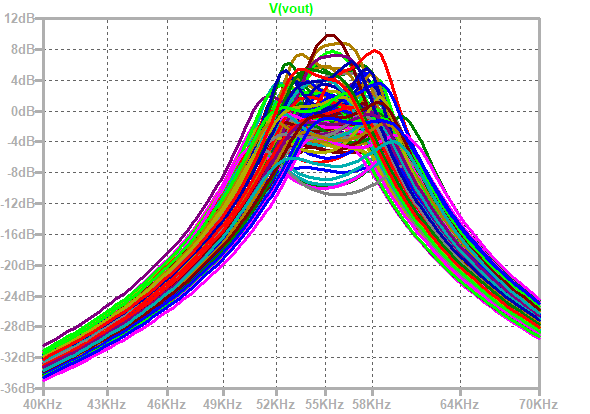
\includegraphics[height=7.5cm]{../Ex2/Informe/montecarlo.png}
\end{center}
\end{figure}


\section{Celda Construida}

\subsection{Selección de componentes}

Se utilizaron los componentes indicados en los Cuadros \ref{tab:e2 comp cell 1} y \ref{tab:e2 comp cell 2} para construir las celdas.

\begin{table}[ht]
\begin{center}
\begin{tabular}{||c|c|c|c||}
\hline
Componente	&	Construcción	&	Valor	&	Unidad	\\
\hline
$R_1/a$	&	$68k + 8.2 k$	&	$76.2 k$	&	$\si{\ohm}$	\\
$R_1/(1-a)$	&	$150k // 2.2 k$	&	$2.17 k$	&	$\si{\ohm}$	\\
$R_2$ &	$18 k + 1 k$	&$19.0k$&	$\si{\ohm}$	\\
$C$	&	$468 p$	&	$468 p$	&	$\si{\farad}$	\\
\hline
\end{tabular}
\caption{Componentes de la primera celda}
\label{tab:e2 comp cell 1}
\end{center}
\end{table}

\begin{table}[ht]
\begin{center}
\begin{tabular}{||c|c|c|c||}
\hline
Componente	&	Construcción	&	Valor	&	Unidad	\\
\hline
$R_1/a$	&	$39k + 820 k$	&	$76.2 k$	&	$\si{\ohm}$	\\
$R_1/(1-a)$	&	$1.5k // 4.7 k$	&	$2.17 k$	&	$\si{\ohm}$	\\
$R_2$ &	$1.8 M // 10 k$	&$19.0k$&	$\si{\ohm}$	\\
$C$	&	$809 p$	&	$809 p$	&	$\si{\farad}$	\\
\hline
\end{tabular}
\caption{Componentes de la segunda celda}
\label{tab:e2 comp cell 2}
\end{center}
\end{table}

Todas las resistencias utilizadas fueron de tecnología SMD ya que las sensibilidades del circuito eran muy altas en todos los parámetros, no sólo de la relación de las resistencias en la retroalimentación positiva. Los capacitores utilizados fueron de tecnología multicapa para la primera celda por su disponibilidad y su respuesta en frecuencia más óptima para este rango de frecuencias. Por otro lado se utilizaron resistencias de tipo \textit{Plate} para la segunda celda ya que para esa capacitancia era la tecnología disponible.

\subsection{Resultados de las Mediciones}

\textit{Los resultados de las mediciones se agregarán más tarde.}

La respuesta en frecuencia fue medida, utilizando un \textit{Analog Discovery}, excitando el circuito con una señal de entrada de amplitud $1 V_{PP}$. La impedancia de entrada, por su lado, fue medida conectando un resistor de $100 \si{\kilo\ohm}$ previo a la entrada del filtro y utilizando el \textit{Analog Discovery} configurado para medir esta impedancia de entrada.

\begin{figure}[ht]
\begin{center}
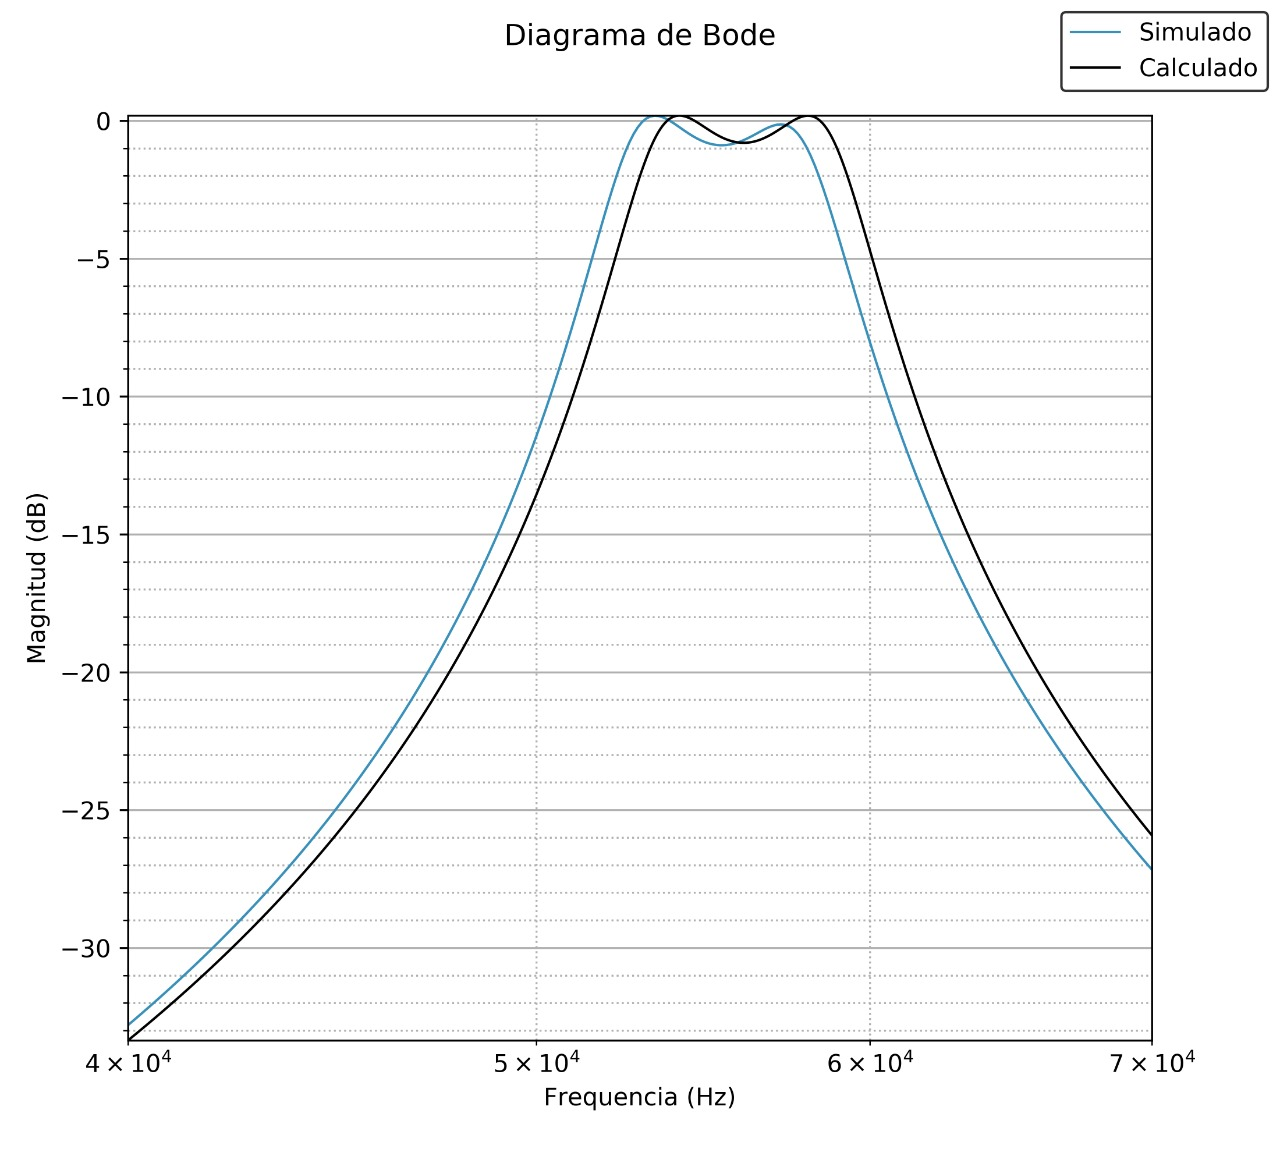
\includegraphics[height=7.5cm]{../Ex2/Informe/TransferenciaTotal.jpeg}
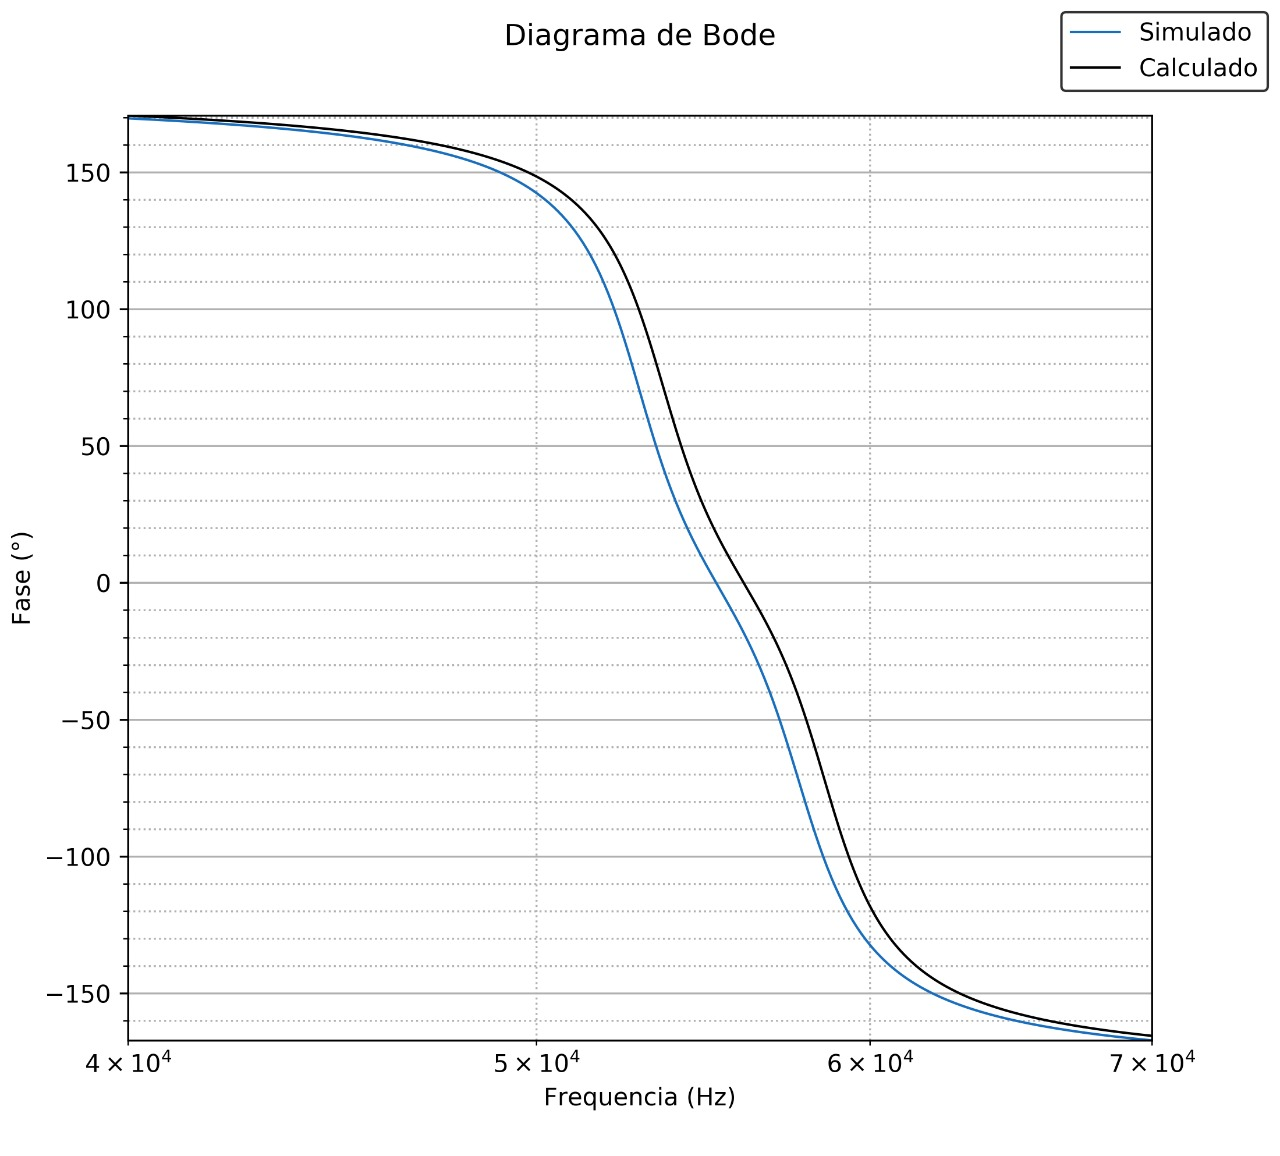
\includegraphics[height=7.5cm]{../Ex2/Informe/FaseTotal.jpeg}
\caption{Transferencia de las Celdas en Cascada}
\label{fig:e2 H total}
\end{center}
\end{figure}

\begin{figure}[ht]
\begin{center}
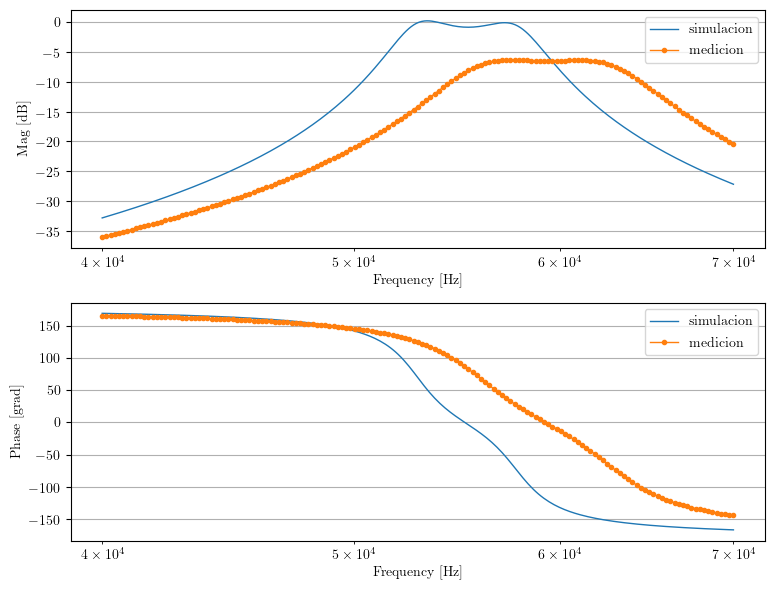
\includegraphics[width=0.7\linewidth]{../Ex2/Informe/simymed.png}
\end{center}
\end{figure}

\begin{figure}[ht]
\begin{center}
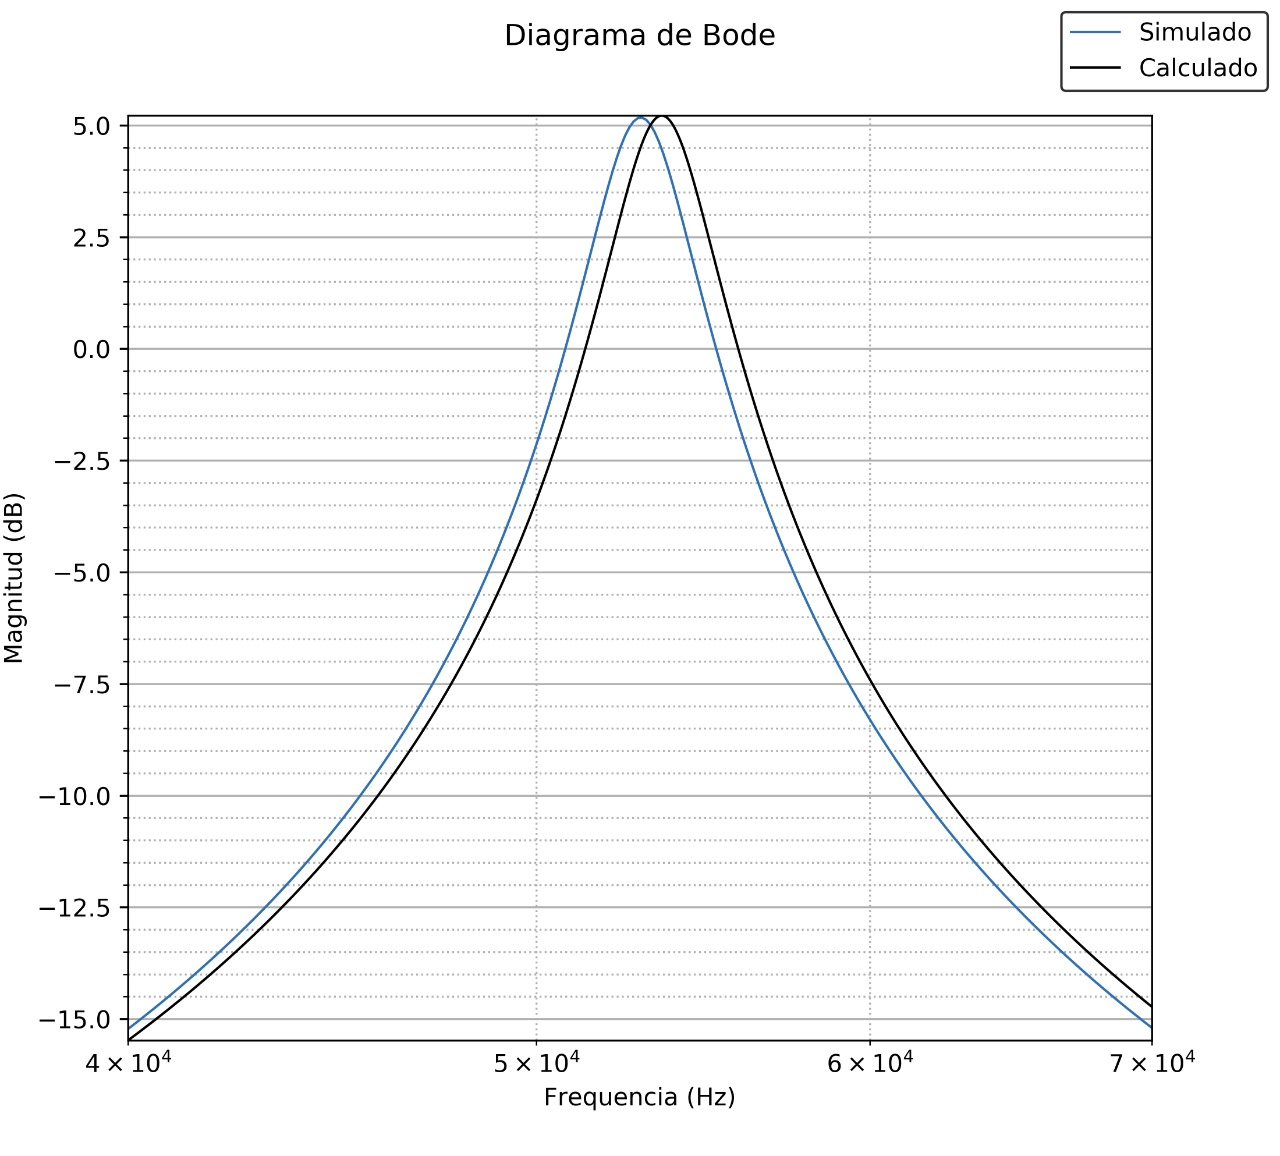
\includegraphics[height=7.5cm]{../Ex2/Informe/TransferenciaCell1.jpeg}
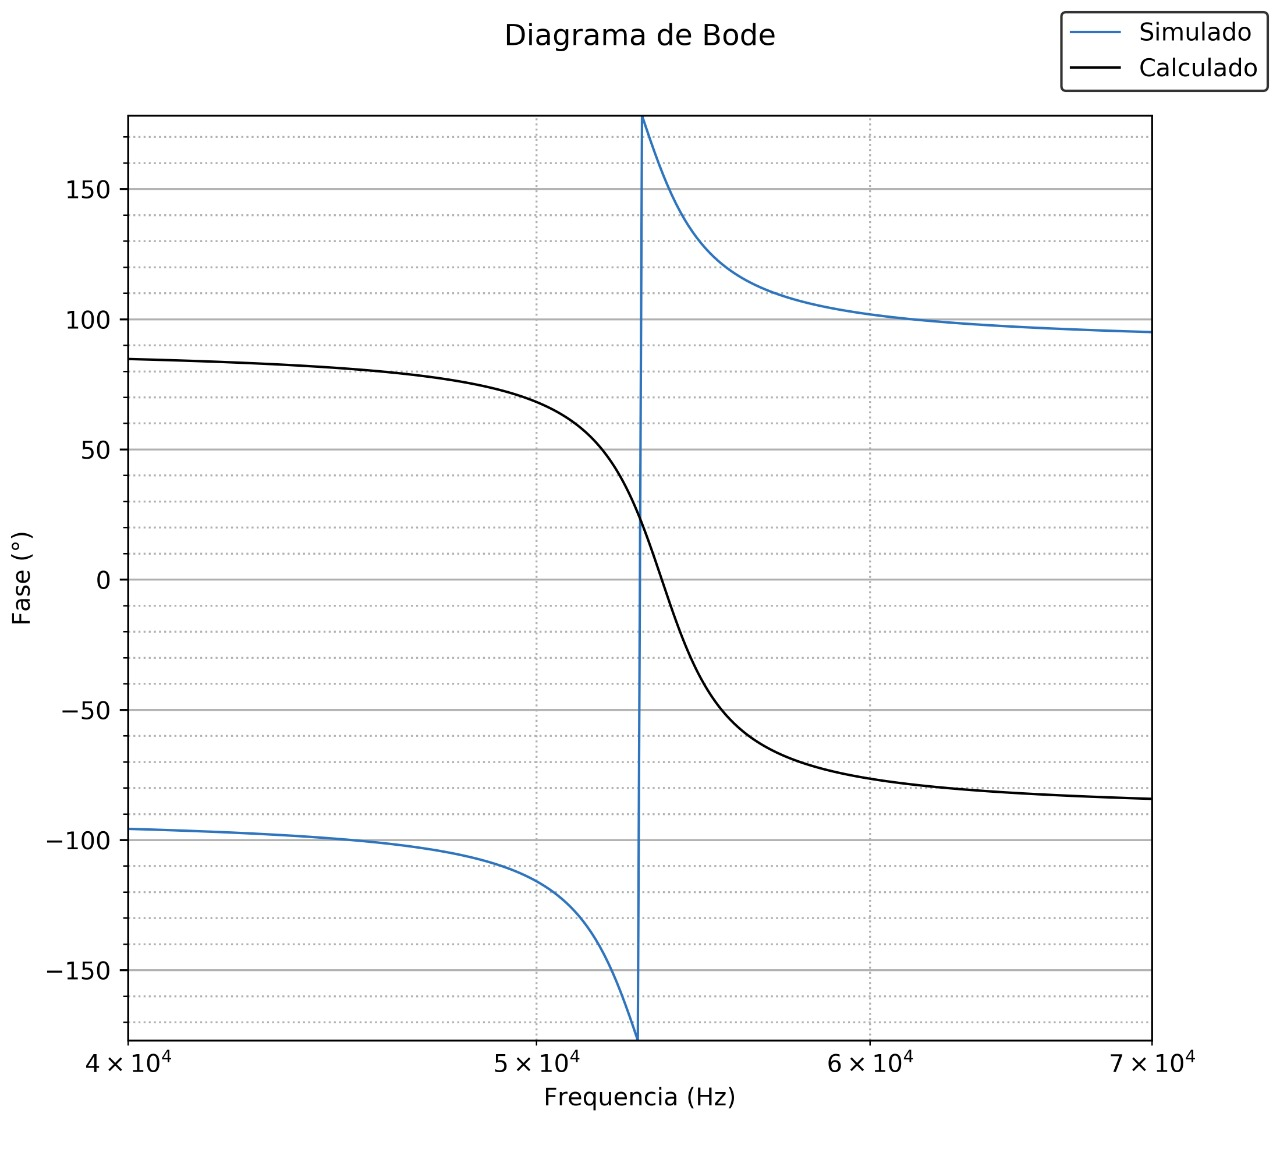
\includegraphics[height=7.5cm]{../Ex2/Informe/FaseCell1.jpeg}
\caption{Transferencia de la primera Celda}
\label{fig:e2 H cell1}
\end{center}
\end{figure}

\begin{figure}[ht]
\begin{center}
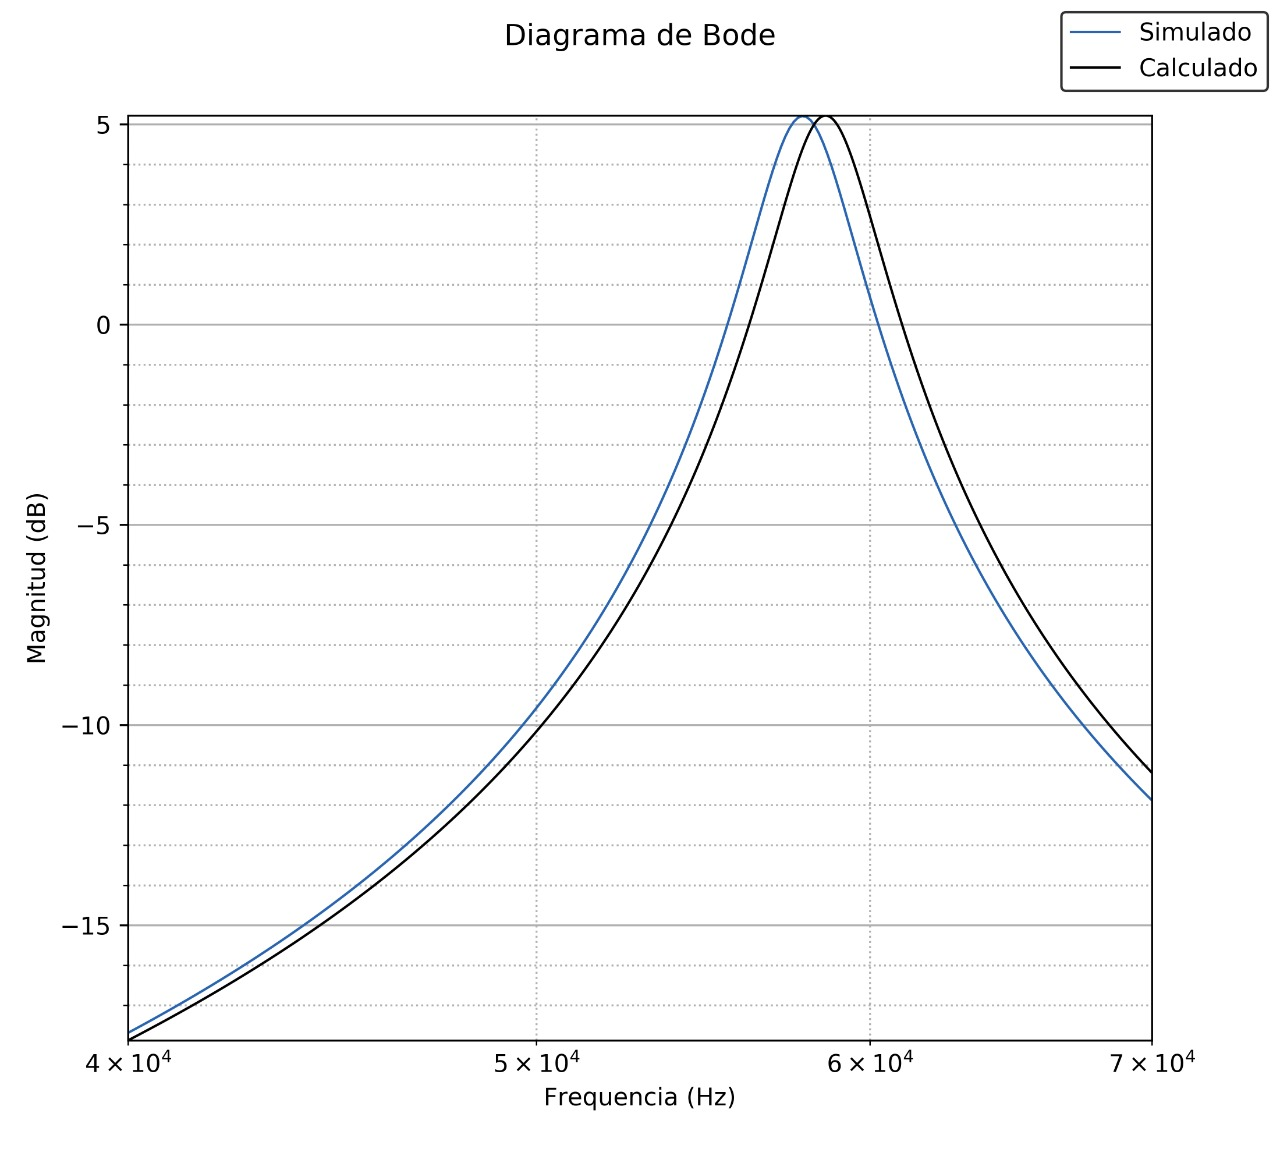
\includegraphics[height=7.5cm]{../Ex2/Informe/TransferenciaCell2.jpeg}
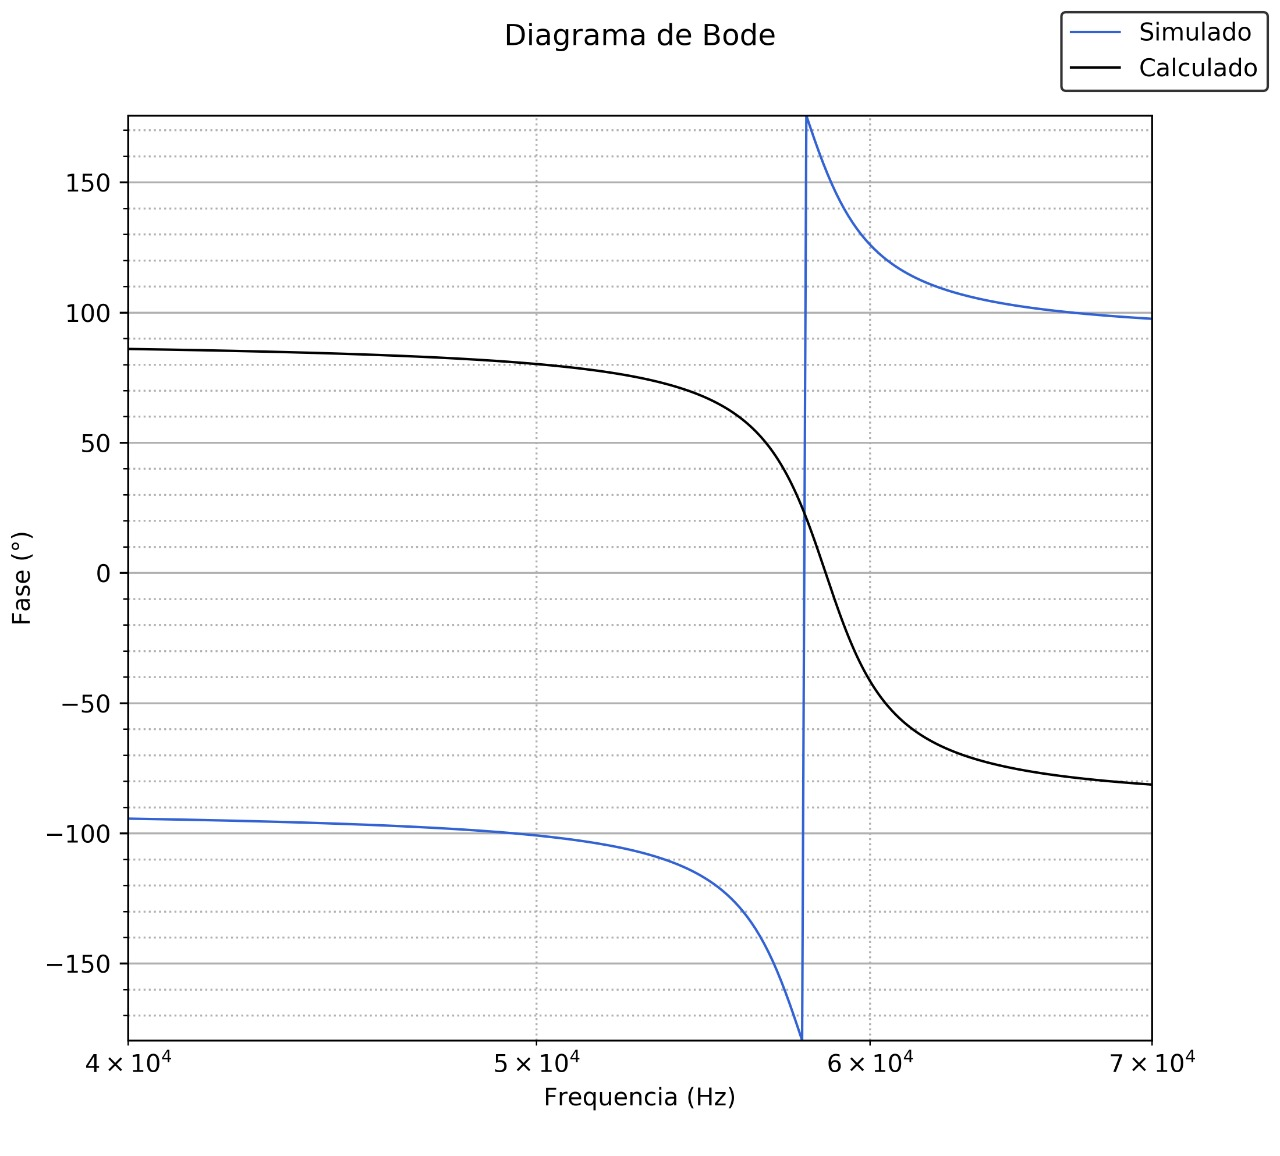
\includegraphics[height=7.5cm]{../Ex2/Informe/FaseCell2.jpeg}
\caption{Transferencia de la segunda Celda}
\label{fig:e2 H cell2}
\end{center}
\end{figure}

\begin{figure}[ht]
\begin{center}
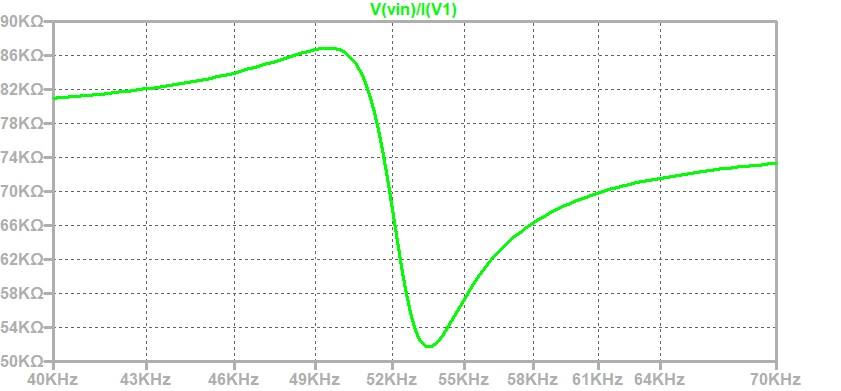
\includegraphics[height=7.5cm]{../Ex2/Informe/Zin.jpg}
\caption{Impedancia de Entrada de las Celdas en Cascada}
\label{fig:e2 Z total}
\end{center}
\end{figure}

%\begin{figure}[ht]
%\begin{center}
%\includegraphics[height=7.5cm]{../Ex2/Informe/ImpedanciaCell1.png}
%\caption{Impedancia de Entrada de la primera Celda}
%\label{fig:e2 Z cell1}
%\end{center}
%\end{figure}
%
%\begin{figure}[ht]
%\begin{center}
%\includegraphics[height=7.5cm]{../Ex2/Informe/ImpedanciaCell2.png}
%\caption{Impedancia de Entrada de la segunda Celda}
%\label{fig:e2 Z cell2}
%\end{center}
%\end{figure}

\subsection{Análisis de los Resultados}

En la figura \ref{fig:e2 H total} se puede observar que no pudo obtenerse una transferencia que corresponda a la plantilla, a pesar que sí se pudo obtener un filtro pasabandas de cuarto orden. Esto puede deberse a que por las altas sensibilidades a los componentes que tienen los parámetros de las celdas, cualquier pequeña desviación en los valores necesarios pueden causar una significante modificación de estos.

En el caso de este filtro, dado que las capacitancias de los componentes son menores a las deseadas, toda la banda pasante se vio desplazada hacia la derecha en el gráfico de la respuesta en frecuencia. La causa de esto es más evidente en los gráficos \ref{fig:e2 H cell1} y \ref{fig:e2 H cell2} donde se puede observar cómo estas capacitancias distintas a las usadas para diseñar la celda causan que las frecuencias centrales de cada pasa banda de primer orden sean desplazadas hacia frecuencias mayores, relación que puede observarse también en el cálculo de la frecuencia central de cada celda.

Por otro lado, la atenuación observada en la transferencia sólo podría ser atribuida a las resistencias utilizadas o a la configuración del preset. Sin embargo, aunque todas estas fueron calibradas de previo a la medición, esta reducción en la amplitud de salida podría ser atribuida a defectos en el amplificador operacional.

Observando la figura \ref{fig:e2 Z total} se puede observar cómo, a pesar que las capacitancias no son iguales a las deseadas, la impedancia de entrada del filtro se siguió manteniendo sobre los $50 \si{\kilo\ohm}$ para todo el rango de frecuencias de la banda pasante.

\subsection{Calibración}

Idealmente si el filtro se encontrase en correcto funcionamiento, con una alimentación de $\pm 15 V$ se debe calibrar el filtro de la siguiente manera:

\begin{itemize}
\item Medir la ganancia en la salida de la primera celda y buscar la frecuencia donde se encuentre el máximo de ganancia. Modificar el preset de esta celda hasta que la ganancia sea de $5 \si{\deci\bel}$.
\item Medir la ganancia en la salida de la segunda celda, conectada en cascada y buscar la otra frecuencia donde se encuentre el otro máximo de la ganancia. Una vez encontrado ajustar el preset de la segunda celda hasta que la ganancia de este punto sea de $0 \si{\deci\bel}$
\item Buscar las frecuencias donde la ganancia sea de $-3 \si{\deci\bel}$ y verificar que estar frecuencias se encuentren dentro de la banda pasante de la plantilla del diseño.
\end{itemize}

\subsection{Rango Dinámico}

Teniendo en cuenta que la máxima ganancia en cualquiera de estas celdas debería ser de $5.1 \si{\deci\bel}\approx 1.8 V/V$, la señal de entrada debe ser tal que no sature la salida de ningún amplificador operacional, principalmente el que pertenece a la primera celda. Dado que se alimenta el integrado con una tensión de $\pm 15 V$ se considera que este saturará con una tensión de $14 V$, por lo tanto:

\begin{equation}
V_{i Max} = \frac{V_{o Max}}{1.8} = 7.78 V
\end{equation}

Considerando una tensión mínima de salida $V_{oMin} = 10 \si{\milli\volt}$ y que la ganancia mínima de este circuito según la plantilla debe ser de
$-3 \si{\deci\bel} \approx 0.708 V/V $:

\begin{equation}
V_{iMin} = \frac{V_{oMin}}{0.708} = 14.1 \si{\milli\volt}
\end{equation}

En conclusión, el rango dinámico de este filtro debería ser:
\begin{equation}
RD = 20 log\left(\frac{V_{i Max}}{V_{i min}} \right)= 54.84 \si{\deci\bel}
\end{equation}

\newpage

\section{Anexo}

\subsection{Transferencia Numérica}

Dado que se utilizó $A_p=1 \si{\deci\bel}$ se obtuvo $\epsilon$ tal que:

\begin{equation}
\epsilon=\sqrt{10^{A_p/10}-1}=\sqrt{10^{0.1}-1} = 0.5088
\end{equation}

Luego se calcularon las singularidades correspondientes al pasabajos normalizado de orden $n=2$:

\begin{equation}
s_P= -\sigma _k  + j \omega _k
\label{eq:e2sing}
\end{equation}

\begin{equation}
\sigma _k=-senh( \beta ) sen(\alpha _k)
\label{eq:e2sigma}
\end{equation}

\begin{equation}
\omega _k=cosh( \beta) cos(\alpha _k)
\label{eq:e2omega}
\end{equation}

\begin{equation}
\alpha_k=\frac{2k-1}{2n}\pi \qquad (0 \leq k \leq 2n-1)
\label{eq:e2alphak}
\end{equation}

\begin{equation}
\beta=senh^{-1}\left( \epsilon^{-1}\right) 
\label{eq:e2beta}
\end{equation}

A partir de las ecuaciones \eqref{eq:e2sigma} a \eqref{eq:e2beta} se obtienen 4 polos (2 pares complejos conjugados). Para el diseño del filtro, se tomaron aquellos en el semiplano izquierdo y se obtuvo la transferencia del pasabajos normalizado:

\begin{equation}
H_{LPN}(s)=\frac{1}{(s-s_{p1})(s-\bar{s_{p1}})}
\label{eq:e2LPN}
\end{equation}

A la expresión \eqref{eq:e2LPN} se le aplicó la desnormalización del pasabajos al pasabanda:

\begin{equation}
s \rightarrow \frac{1}{B}\left(\frac{s}{\omega_0}+\frac{\omega_0}{s}\right)
\label{eq:e2LP2BP}
\end{equation}

Aplicando la desnormalización \eqref{eq:e2LP2BP} se obtuvo la transferencia de 4º orden:

\begin{equation}
H_{BP}(s) = \frac{B^2 \omega_0^2 s}{s^4 + \left(2 \sigma B \omega_0\right) s^3 + \left[ 2+B^2 \left(\sigma^2 + \omega^2 \right) \right] w_o^2 + \left(2 \sigma B \omega_0^3\right) s + w_0^4}
\end{equation}

\begin{equation*}
H_{BP}(s)=\frac{1.2380\cdot10^9s^2}{s^4+3.8625\cdot10^4 s^3+2.4897\cdot10^{11}s^2+4.7819\cdot10^{15}+1.5328\cdot10^{22}}
\end{equation*}

\subsection{Transferencia de la Celda Rauch}

Se calculó la transferencia de la Celda Rauch aplicando la ley de Nodos de Kirchoff y con asistencia de MATLAB.

\begin{figure}[ht]
\begin{center}
\begin{circuitikz}[american voltages]
\draw
(0,0) node[op amp] (opamp) {$A$}
(opamp.-) to[capacitor=$C$,*-*] ++(-3,0) coordinate(tmp) node[above left] {$V_x$}
(tmp) to[resistor=$\frac{R_1}{(1-a)}$] ++(0,-2) node[ground]{}
(tmp) to[resistor=$\frac{R_1}{a}$,-o] ++(-3,0) node[left]{$V_{in}$}
(opamp.out) to[short] ++(0,2) coordinate(tmp1) to [short] ++(0,1.5) coordinate(tmp2)
(tmp1) to[resistor=$R_2$] ++(-2,0) -| (opamp.-)
(tmp2) to[capacitor=$C$] ++(-2,0) -| (tmp)
(opamp.out) to[short,-o] ++(1,0) node[right]{$V_{out}$}
(opamp.out) to[resistor=$R(1-K)$] ++(0,-2) coordinate(vp)
(vp) to[resistor=$RK$] ++(0,-2) node[ground]{}
(vp) -| (opamp.+)
;
\end{circuitikz}
\caption{Celda Rauch con Q mejorado}
\end{center}
\end{figure}

Se aplicó la ley de nodos de Kirchoff en $V_x$ y $V^-$:

\begin{equation}
\mathlarger{
\frac{V_{in}-V_x}{R_1/a}=\frac{V_x-V_{out}}{1/sC}+\frac{V_x}{R_1/(1-a)}+\frac{V_x-V^-}{1/sC}
}
\label{eq:e2vx}
\end{equation}

\begin{equation}
\mathlarger{
\frac{V_x-V^-}{1/sC}=\frac{V^--V_{out}}{R_2}
}
\label{eq:e2v-}
\end{equation}

\begin{equation}
\mathlarger{
V^-=V^+ - \frac{V_{out}}{A} = V_{out} (K - 1/A)
}
\label{eq:e2v-val}
\end{equation}

Además, tomando divisor de tensiones:

\begin{equation}
\mathlarger{
V^+=V_{out}\cdot\frac{KR}{KR+(1-K)R}=V_{out}K
}
\label{eq:e2v+}
\end{equation}

Resolviendo algebráicamente las ecuaciones \eqref{eq:e2vx}, \eqref{eq:e2v-}, \eqref{eq:e2v-val} y \eqref{eq:e2v+} se obtuvo la transferencia de la celda:

\begin{equation}
\mathlarger{
H(s)=-\frac{1}{1-K+1/A} \cdot \frac{\frac{a}{R_1C}s}{s^2 + \frac{2}{R_2 C}\cdot \left(1-\frac{R_2}{2 R_1}\cdot \frac{K-1/A}{1-K+1/A} \right)s + \frac{1}{R_1R_2C^2}}
}
\label{eq:e2 cell avol}
\end{equation}

Aproximando con $A\rightarrow \infty$ para un amplificador operacional ideal, se obtiene la transferencia en \eqref{eq:e2cell}

\subsection{Impedancia de Entrada}

\begin{equation}
i_{in} = \left(V_{in} - V_x \right) / \frac{R_1}{a} = \left( V_{in} - V_{out} \frac{1}{sC} \left[ K(1/R_2 + sC) - 1/R_2 \right]\right)/\frac{R_1}{a}
\end{equation}

\begin{equation*}
i_{in} = V_{in} \left[1- H(s) \frac{1}{sC} \left[ K(1/R_2+sC) - 1/R_2 \right] \right]=V_{in} \left[1+ H(s) \left(\frac{1-K}{sCR_2} - K \right) \right]/\frac{R_1}{a}
\end{equation*}

\begin{equation}
Z_{in} = \frac{V_{in}}{i_{in}}= \frac{R_1/a}{1+H(s) \left(\frac{1-K}{sCR_2} - K \right)}
\end{equation}

Operando algebráicamente se obtiene la expresión

\begin{equation*}
Z_{in} = \frac{R_1}{a} \cdot \frac{s^2 + \frac{\omega_0}{Q}s + \omega_0^2}{s^2 + \frac{\omega_0}{Q}(1-GK) s + \omega_0^2 + \frac{\omega_0}{Q} \frac{G(1-K)}{C R_2}}
\end{equation*}

\subsection{Análisis de Sensibilidades}

Operando sobre las siguientes expresiones:

\begin{equation*}
w_0^2=\frac{1}{R_1R_2C^2} \qquad G_0 = \frac{aR_2}{2R_1} \qquad Q_0=\frac{1}{2}\sqrt{\frac{R_2}{R_1}} \qquad	\alpha=\frac{K}{1-K}
\end{equation*}

\begin{equation*}
Q = \frac{Q_0}{\left(1-2 Q_0^2\alpha\right)} \qquad	G=G_0\cdot\frac{Q}{Q_0}\cdot\frac{1}{1-K}
\end{equation*}

se obtuvieron expresiones en función de los componentes con los cuales se calcula la sensibilidad:

\begin{equation}
\omega_0 = \frac{1}{\sqrt{R_1 R_2}C}
\end{equation}

\begin{equation}
Q=\frac{1}{2} \sqrt{\frac{R_2}{R_1}} \frac{R_1(1-K)}{2R_1-K(2R_1+R_2)}
\end{equation}

\begin{equation}
G=a\frac{R_2}{2R_1-K(2R_1+R_2)}
\end{equation}

Para poder calcular las sensibilidades de los parámetros $\omega_0$, $Q$, y $G$ respecto a $A_{VOL}$ se obtuvieron sus funciones a partir de la expresión \eqref{eq:e2 cell avol}

\begin{equation}
Q (R_1,R_2,K,A)= \frac{0.5 \sqrt{R_2/R_1}}{1 - \frac{R_2}{2R_1}\cdot \frac{K-1/A}{1-K+1/A}}
\end{equation}

\begin{equation}
G (R_1,R_2,K,A,a) = \frac{a R_2}{2R_1-(K-1/A)(2R_1+R_2)}
\end{equation}

Se calcularon las derivadas sensibilidades de cada parámetro respecto a sus componentes utilizando expresiones simbólicas en MATLAB y operando algebráicamente:

\begin{table}[ht]
\begin{center}
\begin{tabular}{||c|c|c|c||}
\hline
$f(...)$			&	$\omega_0$	&	$Q$	&	$G$	\\
\hline
\hline
$S_{R1}^f$	&	$-0.5$	&	$-\frac{K R_2}{2R_1(1-K)-KR_2}-\frac{1}{2}$	&	$-\frac{2R_1(1-K)}{2R_1(1-K)-KR_2}$\\
\hline
$S_{R2}^f$	&	$-0.5$	&	$\frac{K R_2}{2R_1(1-K)-KR_2}+\frac{1}{2}$	&	$\frac{2R_1(1-K)}{2R_1(1-K)-KR_2}$\\
\hline
$S_{C}^f$		&	$-1$	&	$0$	&	$0$	\\
\hline
$S_{K}^f$		&	$0$	&	$\frac{KR_2(1-K)}{2R_1(1-K)-KR_2}$	&	 $\frac{2R_1}{2R_1-K(2R_1+R_2)}-1$\\
\hline
$S_{A}^f$		&	$0$	&	$\frac{1}{A}\cdot\frac{R_2}{(1-K+1/A)[2R_1 + (R_2+2R_1)(1/A-K)]}$& $\frac{1}{A}\cdot\frac{R_2+2R_1}{(R_2+2R_1)(1/A-K)+2R_1}$	\\
\hline
$S_{a}^f$		&	$0$	&	$0$	&	$1$	\\
\hline
\end{tabular}
\caption{Sensibilidades de los parámetros en una celda}
\label{tab:e2 sens gen}
\end{center}
\end{table}

